\documentclass{article}

\usepackage{amsmath, amsthm, amssymb, amsfonts}
\usepackage{thmtools}
\usepackage{pgfplots}
\pgfplotsset{compat=1.17}

\usepackage{tikz}
\usepackage{graphicx}
\usepackage{setspace}
\usepackage{geometry}
\usepackage{float}
\usepackage{hyperref}
\usepackage[utf8]{inputenc}
\usepackage[english]{babel}
\usepackage{framed}
\usepackage[dvipsnames]{xcolor}
\usepackage{tcolorbox}
\usepackage[table,xcdraw]{xcolor}
\tcbset{terminal/.style={
  colback=black, coltext=green, colframe=black,
  listing only, listing options={language=bash, basicstyle=\ttfamily}
}}
\usepackage{qrcode}      % For QR codes
\definecolor{spotifygreen}{RGB}{30,215,96} % Official Spotify Green
\usepackage{fontawesome5} % For Spotify icon and other FontAwesome 5 icons


\colorlet{LightGray}{White!90!Periwinkle}
\colorlet{LightOrange}{Orange!15}
\colorlet{LightGreen}{Green!15}

\newcommand{\HRule}[1]{\rule{\linewidth}{#1}}

\declaretheoremstyle[name=Theorem,]{thmsty}
\declaretheorem[style=thmsty,numberwithin=section]{theorem}
\tcolorboxenvironment{theorem}{colback=white}

\declaretheoremstyle[name=Corollary,]{thmsty}
\declaretheorem[style=thmsty,numberwithin=section]{corollary}
\tcolorboxenvironment{corollary}{colback=white}

\declaretheoremstyle[name=Theorem,]{thmsty}
\declaretheorem[style=thmsty,numberwithin=section]{subtheorem}
\tcolorboxenvironment{subtheorem}{colback=white}

\declaretheoremstyle[name=Proposition,]{prosty}
\declaretheorem[style=prosty,numberwithin=section]{proposition}
\tcolorboxenvironment{proposition}{colback=white}

\declaretheoremstyle[name=Principle,]{prcpsty}
\declaretheorem[style=prcpsty,numberlike=theorem]{principle}
\tcolorboxenvironment{principle}{colback=white}

\setstretch{1.2}
\geometry{
    textheight=9in,
    textwidth=5.5in,
    top=1in,
    headheight=12pt,
    headsep=25pt,
    footskip=30pt
}

% ------------------------------------------------------------------------------

\begin{document}

% ------------------------------------------------------------------------------
% Cover Page and ToC
% ------------------------------------------------------------------------------

\title{ \normalsize \textsc{}
		\\ [0cm]
		\HRule{1.5pt} \\
		\LARGE \noindent \textbf{\uppercase{Calculus \& analytical geometry (2)\\ (MATH 132)-Worksheet\#01}
		\HRule{2.0pt} \\ [0.6cm] \LARGE{Cairo University \\ Faculty Of Science} \vspace*{1\baselineskip}}
        \\
        
		}
        
\date{$2^{\text{nd}}$ week (February 15, 2025 - February 20, 2025)}

\author{ \noindent \textbf{Written \& Reviewed by} \\ 3ndlyb Alabyd} \\ 

\maketitle


\section*{Answer for OLD Q1}
\label{sec:Q1}

We are given the function  
\[
f(x) = 1 - x^3,
\]
and the region \( S \) bounded by the graph of \( f \), the vertical lines \( x = 1 \) and \( x = 5 \), and the \( x \)-axis.

\subsection*{Step 1: Understanding the Region}  

Notice that  
\[
f(1) = 1 - 1^3 = 0,
\]
and for \( x > 1 \),  
\[
f(x) = 1 - x^3 < 0.
\]
Thus, for \( x \) in \([1,5]\), the curve \( y = f(x) \) lies below the \( x \)-axis. The note in the \textit{lecture 1} file states:
\begin{quote}
``If \( f \) is a decreasing function, then left endpoints give overestimation."
\end{quote}


Since \( f(x) \) is decreasing on \([1,5]\), using the left endpoints will provide an overestimate.

\subsection*{Step 2: Setting Up the Riemann Sum}  

We approximate the signed area using 4 rectangles. The interval \([1,5]\) has length  
\[
5 - 1 = 4,
\]
so the width of each rectangle is  
\[
\Delta x = \frac{4}{4} = 1.
\]

The 4 subintervals are:  
\[
[1,2],\quad [2,3],\quad [3,4],\quad [4,5].
\]

Since \( f \) is decreasing, we use the left endpoint of each subinterval to compute the height of the rectangle. The left endpoints are:  
\[
x_0 = 1,\quad x_1 = 2,\quad x_2 = 3,\quad x_3 = 4.
\]

\subsection*{Step 3: Evaluating \( f \) at the Left Endpoints}  

Compute the function values:
\begin{align*}
f(1) &= 1 - 1^3 = 0, \\
f(2) &= 1 - 2^3 = 1 - 8 = -7, \\
f(3) &= 1 - 3^3 = 1 - 27 = -26, \\
f(4) &= 1 - 4^3 = 1 - 64 = -63.
\end{align*}

\subsection*{Step 4: Compute $ L_4 $ Approximation}  

The area (signed) for each rectangle is given by the height times the width. Thus, the left-endpoint sum is  
\[
L_4 = \Delta x \cdot \big[f(1) + f(2) + f(3) + f(4)\big].
\]
Substituting the values:  
\[
L_4 = 1 \cdot (0 + (-7) + (-26) + (-63)) = 0 - 7 - 26 - 63=-96.
\]


Thus, the upper estimation for the signed area is  
\[
\boxed{S \approx L_4 =-96}.
\] 
\newpage
The estimated signed area using the left-endpoint method is \(-96\), while the right-endpoint estimate gives \(-220\).\footnote{In the \S \hyperref[sec:Q1]{OLD Q1}, we consider the \textbf{signed} area, meaning areas below the \( x \)-axis are negative. Since \( f(x) = 1 - x^3 \) is decreasing on \([1,5]\), the left-endpoint sum results in a \textbf{less negative} value, making it an \textbf{overestimate}. However, if we considered the \textbf{absolute} area (where all areas are treated as positive), the situation would be reversed: the left-endpoint sum would be smaller, and the right-endpoint sum would be the overestimate.}

\begin{center}
    \textbf{Graph of } \( f(x) = 1 - x^3 \) \textbf{ with Left and Right Endpoint Rectangles}
\end{center}

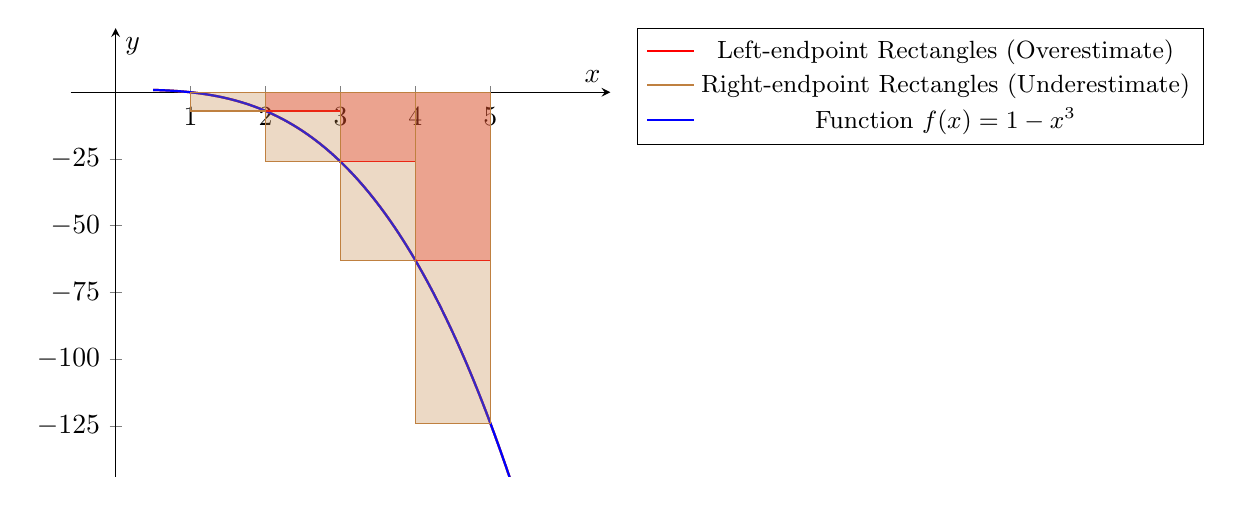
\begin{tikzpicture}
    \begin{axis}[
        axis x line=middle, 
        axis y line=middle, 
        enlargelimits=true,
        xtick={1,2,3,4,5},
        ytick={-125,-100,-75,-50,-25,0},
        xlabel={$x$},
        ylabel={$y$},
        samples=100,
        domain=0.5:5.5,
        ymin=-130
        , ymax=10,
        xmin=0, xmax=6,
        legend style={at={(1.05,1)}, anchor=north west, font=\small}
    ]
    
    % Plot the function

    \addplot[thick,red] {1 - x^3} node[right] {};
    \addlegendentry{Left-endpoint Rectangles (Overestimate)}
    \addplot[thick,brown] {1 - x^3} node[right] {};
    \addlegendentry{Right-endpoint Rectangles (Underestimate)}
    \addplot[thick,blue] {1 - x^3} node[right] {};
    \addlegendentry{Function $f(x) = 1 - x^3$}    
    
    % Left-endpoint rectangles (overestimate)
    \foreach \x in {1,2,3,4} {
        \addplot [
            fill=red, fill opacity=0.3,
            draw=red
        ] coordinates {(\x, 0) (\x, {1 - \x^3}) (\x+1, {1 - \x^3}) (\x+1, 0)} -- cycle;
    }


    % Right-endpoint rectangles (underestimate)
    \foreach \x in {2,3,4,5} {
        \addplot [
            fill=brown, fill opacity=0.3,
            draw=brown
        ] coordinates {(\x, 0) (\x, {1 - \x^3}) (\x-1, {1 - \x^3}) (\x-1, 0)} -- cycle;
    }

    
    \end{axis}
\end{tikzpicture}
\section*{Answer for NEW Q1}
To estimate the area of the region $S$ bounded by the curves $f(x) = 1 - x^3$, the lines $x = -5$ and $x = -1$, and the $x$-axis, we follow these steps:

\subsection*{Step 1: Determine the Interval and Subintervals}
We divide the total width of the interval:
\[
-1 - (-5) = 4
\]
into 4 equal subintervals:
\[
\Delta x = \frac{4}{4} = 1
\]
Thus, the subintervals are:
\[
[-5, -4], [-4, -3], [-3, -2], [-2, -1]
\]

\subsection*{Step 2: Determine Whether $f(x)$ is Decreasing}
To check whether $f(x)$ is decreasing, we compute its derivative:
\[
f'(x) = \frac{d}{dx} (1 - x^3) = -3x^2
\]
Since $x^2 \geq 0$ for all $x$, it follows that:
\[
-3x^2 \leq 0, \quad \text{and for any } x \neq 0, \quad f'(x) < 0
\]
This confirms that $f(x)$ is strictly decreasing for all $x$, including on the given interval $[-5, -1]$.

\subsection*{Step 3: Use Left Endpoints for Overestimation}
Since $f(x)$ is decreasing, the function values at the left endpoints provide an \textbf{overestimate} of the actual area.

The left endpoints are $x = -5, -4, -3, -2$, and evaluating $f(x)$ at these points:
\[
f(-5) = 1 - (-5)^3 = 1 + 125 = 126
\]
\[
f(-4) = 1 - (-4)^3 = 1 + 64 = 65
\]
\[
f(-3) = 1 - (-3)^3 = 1 + 27 = 28
\]
\[
f(-2) = 1 - (-2)^3 = 1 + 8 = 9
\]

\subsection*{Step 4: Compute the Upper Sum}
Each rectangle has width $\Delta x = 1$, so the upper estimate for the area is:
\[
S \approx \sum_{i=1}^{4} f(x_i) \cdot \Delta x
\]
\[
S \approx (126 + 65 + 28 + 9) \times 1
\]
\[
S \approx 126 + 65 + 28 + 9 = 228
\]

Thus, the upper estimation for the area of $S$ using 4 rectangles is \textbf{228 square units}.
\begin{center}
    \textbf{Graph of $f(x) = 1 - x^3$ with Left and Right Endpoint Rectangles}
\end{center}

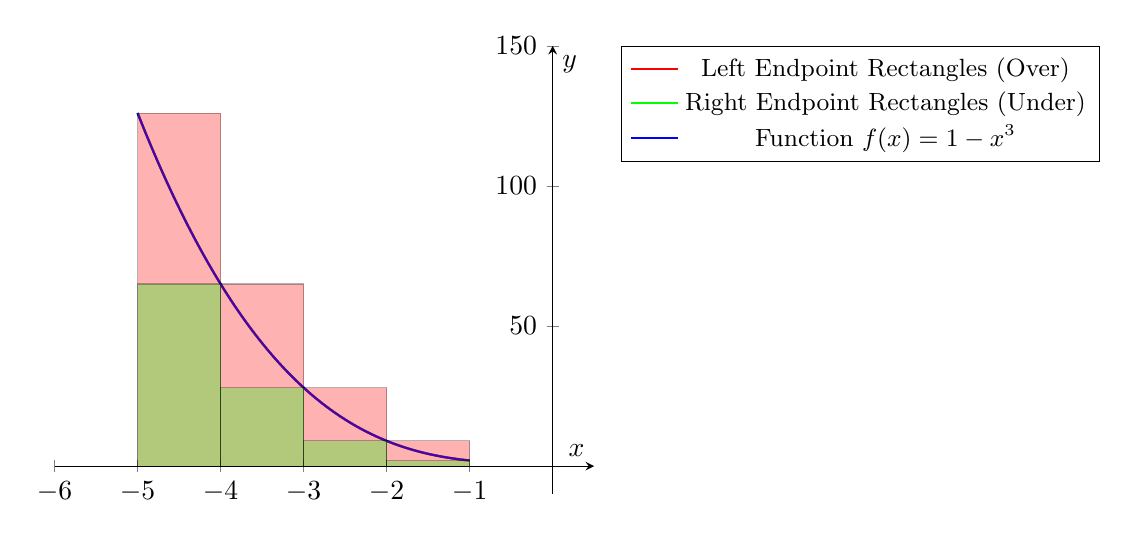
\begin{tikzpicture}
    \begin{axis}[ 
        axis lines = middle, 
        xlabel = {$x$}, 
        ylabel = {$y$}, 
        ymin = -10, ymax = 150, 
        xmin = -6, xmax = 0.5,
        samples=100,
        domain=-5:-1,
        legend style={at={(1.05,1)}, anchor=north west, font=\small}
    ]
        % Plot the function
        
        \addplot[red, thick] {1 - x^3};
        \addlegendentry{Left Endpoint Rectangles (Over)}
        \addplot[green, thick] {1 - x^3};
        \addlegendentry{Right Endpoint Rectangles (Under)}
        \addplot[blue, thick] {1 - x^3};
        \addlegendentry{Function $f(x)=1-x^3$}
        % Left endpoint rectangles (Overestimation)
        \foreach \x in {-5,-4,-3,-2} {
            \addplot [fill=red, opacity=0.3] coordinates {(\x,0) (\x,{1 - \x^3}) (\x+1,{1 - \x^3}) (\x+1,0)} --cycle;
        }

        

        % Right endpoint rectangles (Underestimation)
        \foreach \x in {-5,-4,-3,-2} {
            \addplot [fill=green, opacity=0.3] coordinates {(\x,0) (\x,{1 - (\x + 1)^3}) (\x+1,{1 - (\x + 1)^3}) (\x+1,0)} --cycle;
        }

        
    \end{axis}
\end{tikzpicture}

\section*{Answer of Q2}
Let the given function be:
\[
f(x) = \frac{1}{3 + x^2}
\]
The region is bounded by \( x = -2 \), \( x = -1 \), and the x-axis. We approximate the area using 3 rectangles.

\subsection*{Step 1: Compute the Partition Width}
The interval is \([-2, -1]\) and we divide it into 3 subintervals:
\[
\Delta x = \frac{-1 - (-2)}{3} = \frac{1}{3}
\]
The left endpoints are given by:
\[
x_k = x_0 + k\Delta x, \quad \text{for } k = 0,1,2
\]
where \( x_0 = -2 \).

\subsection*{Step 2: Compute the Left Endpoints}
\begin{align*}
x_0 &= -2, \\
x_1 &= -2 + \frac{1}{3} = -\frac{5}{3}, \\
x_2 &= -2 + \frac{2}{3} = -\frac{4}{3}
\end{align*}

\subsection*{Step 3: Compute Function Values at Left Endpoints}
\begin{align*}
f(x_0) &= f(-2) = \frac{1}{3 + 4} = \frac{1}{7}, \\
f(x_1) &= f\left(-\frac{5}{3} \right) = \frac{1}{3 + \frac{25}{9}} = \frac{1}{\frac{52}{9}} = \frac{9}{52}, \\
f(x_2) &= f\left(-\frac{4}{3} \right) = \frac{1}{3 + \frac{16}{9}} = \frac{1}{\frac{43}{9}} = \frac{9}{43}
\end{align*}

\subsection*{Step 4: Compute \( L_3 \) Approximation for $S$}
\[
L_3 = \sum_{k=1}^{3} f(x_{k-1}) \Delta x
\]
\[
L_3 = \left( \frac{1}{7} + \frac{9}{52} + \frac{9}{43} \right) \times \frac{1}{3}
\]
Converting to a common denominator:
\begin{align*}
\frac{1}{7} &= \frac{52}{364}, \\
\frac{9}{52} &= \frac{63}{364}, \\
\frac{9}{43} &= \frac{81}{364}
\end{align*}

\[
\frac{52}{364} + \frac{63}{364} + \frac{81}{364} = \frac{196}{364}
\]
\[
\boxed{L_3 = \frac{196}{364} \times \frac{1}{3} = \frac{196}{1092}}
\]

Thus, the lower estimation for the area of \( S \) using \( L_3 \) is \textit{approximately} $\frac{196}{1092}$.
\begin{center}
    \textbf{Graph of } \( f(x) = \frac{1}{3 + x^2} \) \textbf{ with Left and Right Endpoint Rectangles}
\end{center}

\begin{tikzpicture}
    \begin{axis}[
        axis x line=middle, 
        axis y line=middle, 
        enlargelimits=true,
        xtick={-3, -2.333, -1.666, -1},
        ytick={0, 0.1, 0.2 },
        xlabel={$x$},
        ylabel={$y$},
        samples=100,
        domain=-3.2:-0.8,
        ymin=,0
        ymax=0.3,
        xmin=-3,
        xmax=0,
        legend style={at={(1.05,1)}, anchor=north west, font=\small}
    ]
    
    % Plot the function
    \addplot[thick,brown] {1/(3 + x^2)} node[right] {};
    \addplot[thick,red] {1/(3 + x^2)} node[right] {};
    \addplot[thick,blue] {1/(3 + x^2)} node[right] {};
    \addlegendentry{\textcolor{brown}{Right-endpoint Rectangles}}
    \addlegendentry{\textcolor{red}{Left-endpoint Rectangles}}
    \addlegendentry{Function \( f(x) = \frac{1}{3 + x^2} \)}
    
    % Left-endpoint rectangles
    \foreach \x in {-3, -2.333, -1.666} {
        \addplot [
            fill=red, fill opacity=0.3,
            draw=red
        ] coordinates {(\x, 0) (\x, {1/(3 + (\x)^2)}) (\x+0.666, {1/(3 + (\x)^2)}) (\x+0.666, 0)} -- cycle;
    }

    % Right-endpoint rectangles
    \foreach \x in {-2.333, -1.666, -1} {
        \addplot [
            fill=brown, fill opacity=0.3,
            draw=brown
        ] coordinates {(\x, 0) (\x, {1/(3 + (\x)^2)}) (\x-0.666, {1/(3 + (\x)^2)}) (\x-0.666, 0)} -- cycle;
    }
    
    
    \end{axis}
\end{tikzpicture}

\section*{Answer of OLD Q3}
We need to lower estimate the area under the curve  
\[
f(x) = x^2 - 3x + 4
\]
over the interval \([0,4]\) using 4 rectangles. 

\subsection*{Step 1: Identify Where \( f(x) \) is Increasing or Decreasing}
We compute the derivative:
\[
f'(x) = 2x - 3.
\]
Setting \( f'(x) = 0 \) to find the critical point:
\[
2x - 3 = 0 \Rightarrow x = \frac{3}{2}.
\]
- \( f(x) \) is \textbf{decreasing} on \( [0, \frac{3}{2}] \).\\
- \( f(x) \) is \textbf{increasing} on \( [\frac{3}{2},4] \).\\

Thus, we break the interval at \( x = \frac{3}{2} \) and approximate separately:\\
- On \( [0, \frac{3}{2}] \), we use \( R_2 \) (right endpoints give the lower estimate).\\
- On \( [\frac{3}{2}, 4] \), we use \( L_2 \) (left endpoints give the lower estimate).\\

\subsection*{Step 2: Compute \( R_2 \) on \( [0, \frac{3}{2}] \)}
Divide \( [0, \frac{3}{2}] \) into 2 equal subintervals:
\[
\left[0, \frac{3}{4} \right], \quad \left[ \frac{3}{4}, \frac{3}{2} \right]
\]
- Width of each rectangle: \( \Delta x = \frac{3}{4} \).\\
- Right endpoints: \( x = \frac{3}{4} \) and \( x = \frac{3}{2} \).\\


Evaluate \( f(x) \) at these points:

\[
f\left(\frac{3}{4}\right) = \left(\frac{3}{4}\right)^2 - 3\left(\frac{3}{4}\right) + 4 = \frac{37}{16}.
\]
\[
f\left(\frac{3}{2}\right) = \left(\frac{3}{2}\right)^2 - 3\left(\frac{3}{2}\right) + 4 = \frac{9}{4} - \frac{9}{2} + 4 = \frac{16}{4} - \frac{18}{4} + \frac{9}{4} = \frac{7}{4}.
\]
Now, approximate the area using \( R_2 \):
\[
R_2 = \Delta x\sum_{i=1}^2 f(x_i) = \left(\frac{3}{4}\right) \left(\frac{37}{16} +  \frac{7}{4}\right)
\]
\[
= \left(\frac{3}{4}\right)\left(\frac{65}{16}\right) = \frac{195}{64}.
\]


\subsection*{Step 3: Compute \( L_2 \) on \( [\frac{3}{2},4] \)}
Divide \( [\frac{3}{2}, 4] \) into 2 equal subintervals:
\[
\left[\frac{3}{2}, \frac{11}{4} \right], \quad \left[\frac{11}{4}, 4 \right]
\]
- Width of each rectangle: \( \Delta x = \frac{5}{4} \).\\
- Left endpoints: \( x = \frac{3}{2} \) and \( x = \frac{11}{4} \).\\

We already have:
\[
f\left(\frac{3}{2}\right) = \frac{7}{4}.
\]
Now, evaluate \( f(x) \) at \( x = \frac{11}{4} \):
\[
f\left(\frac{11}{4}\right) = \frac{53}{16}.
\]

Now, approximate the area using \( L_2 \):
\[
L_2  =\Delta x\sum_{i=1}^2 f(x_{i-1}) = \left(\frac{7}{4} +  \frac{53}{16}\right)
\]
\[
= \left(\frac{5}{4}\right)\left( \frac{81}{16}\right) = \frac{405}{64}.
\]


\subsection*{Step 4: Compute $S$ Area}
\[
\boxed{S \approx R_2 + L_2 = \frac{195}{64} + \frac{405}{64} = \frac{600}{64} = \mathbf{9.375}.}
\]
\\
\begin{center}
    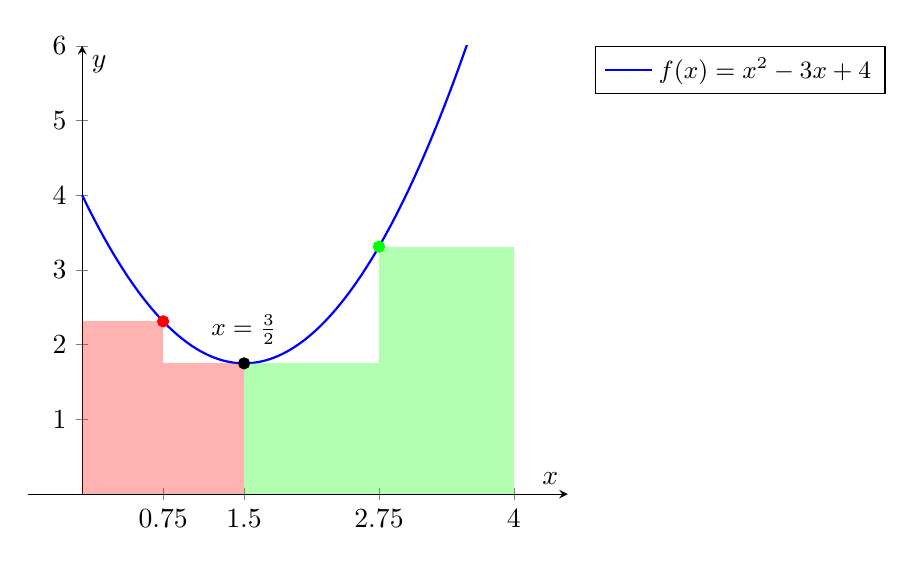
\begin{tikzpicture}
        \begin{axis}[
            axis lines = middle,
            xmin=-0.5, xmax=4.5,
            ymin=0, ymax=6,
            xlabel=$x$, ylabel=$y$,
            samples=100,
            domain=0:4,
            xtick={0,3/4,3/2,11/4,4},
            ytick={1,2,3,4,5,6},
            legend style={at={(1.05,1)}, anchor=north west, font=\small}
        ]

        % Plot function f(x) = x^2 - 3x + 4
        \addplot[blue, thick] {x^2 - 3*x + 4};
        \addlegendentry{$f(x) = x^2 - 3x + 4$}

        % First two rectangles using right endpoints (R_2)
        \fill[red, opacity=0.3] (0,0) rectangle (3/4,37/16);
        \fill[red, opacity=0.3] (3/4,0) rectangle (3/2,7/4);

        % Second two rectangles using left endpoints (L_2)
        \fill[green, opacity=0.3] (3/2,0) rectangle (11/4,7/4);
        \fill[green, opacity=0.3] (11/4,0) rectangle (4,53/16);

        % Add points for right and left endpoints
        \addplot[only marks, mark=*, red] coordinates {(3/4,37/16) };
        \addplot[only marks, mark=*, green] coordinates { (11/4,53/16)};

        % Legend for rectangles
        

        % Critical point marker
        \addplot[only marks, mark=*, black] coordinates {(3/2,7/4)};
        \node at (axis cs:3/2,2.2) {\small $x=\frac{3}{2}$};
        
    \end{axis}
    \end{tikzpicture}
\end{center}
\section*{Answer of NEW Q3}

Let \( S \) be the region bounded between the curves:
\[
f(x) = x^2 - 3x + 4, \quad x = 2, \quad x = 6, \quad \text{and the } x\text{-axis}.
\]
Find the lower estimation for the area of \( S \) using 4 rectangles.
\subsection*{Step 1: Identify the Interval and Number of Rectangles}
\begin{itemize}
    \item The smallest point (lower bound) is \( a = 2 \).
    \item The largest point (upper bound) is \( b = 6 \).
    \item The number of rectangles is \( n = 4 \).
\end{itemize}

\subsection*{Step 2: Compute \(\Delta x\)}
The width of each rectangle is given by:
\[
\Delta x = \frac{b - a}{n} = \frac{6 - 2}{4} = \frac{4}{4} = 1.
\]

\subsection*{Step 3: Determine the \( x_i \) Values}
The endpoints are given by:
\[
x_i = a + i\Delta x
\]
For \( i = 0,1,2,3,4 \):
\[
x_0 = 2, \quad x_1 = 3, \quad x_2 = 4, \quad x_3 = 5, \quad x_4 = 6.
\]

\subsection*{Step 4: Evaluate \( f(x) \) at the Required Points}
The function is:
\[
f(x) = x^2 - 3x + 4.
\]

Evaluating at the chosen points:
\[
f(2) = 2^2 - 3(2) + 4 = 4 - 6 + 4 = 2.
\]
\[
f(3) = 3^2 - 3(3) + 4 = 9 - 9 + 4 = 4.
\]
\[
f(4) = 4^2 - 3(4) + 4 = 16 - 12 + 4 = 8.
\]
\[
f(5) = 5^2 - 3(5) + 4 = 25 - 15 + 4 = 14.
\]
\[
f(6) = 6^2 - 3(6) + 4 = 36 - 18 + 4 = 22.
\]

\subsection*{Step 5: Determine if \( f(x) \) is Increasing or Decreasing}
Differentiate \( f(x) \):
\[
f'(x) = 2x - 3.
\]

Check the sign of \( f'(x) \) on the interval \([2,6]\):
\[
f'(2) = 2(2) - 3 = 1 > 0.
\]

Since \( f'(x) > 0 \) for all \( x \in [2,6] \), \( f(x) \) is \textbf{increasing} on the interval.


\subsection*{Step 7: Compute the Lower Estimation \( L_4 \)}
For an increasing function:
\begin{itemize}
    \item Left endpoint approximation gives the \textbf{lower estimation}.
\end{itemize}
Thus, we will use the left endpoint method.\\

The left endpoint approximation with 4 rectangles is given by:
\[
L_4 = \sum_{k=1}^4 f(x_{k-1}) \Delta x.
\]

Substituting the values:
\[
L_4 = [f(2) + f(3) + f(4) + f(5)] \times 1
\]
\[
L_4 = (2 + 4 + 8 + 14) \times 1
\]
\[
L_4 = 28.
\]


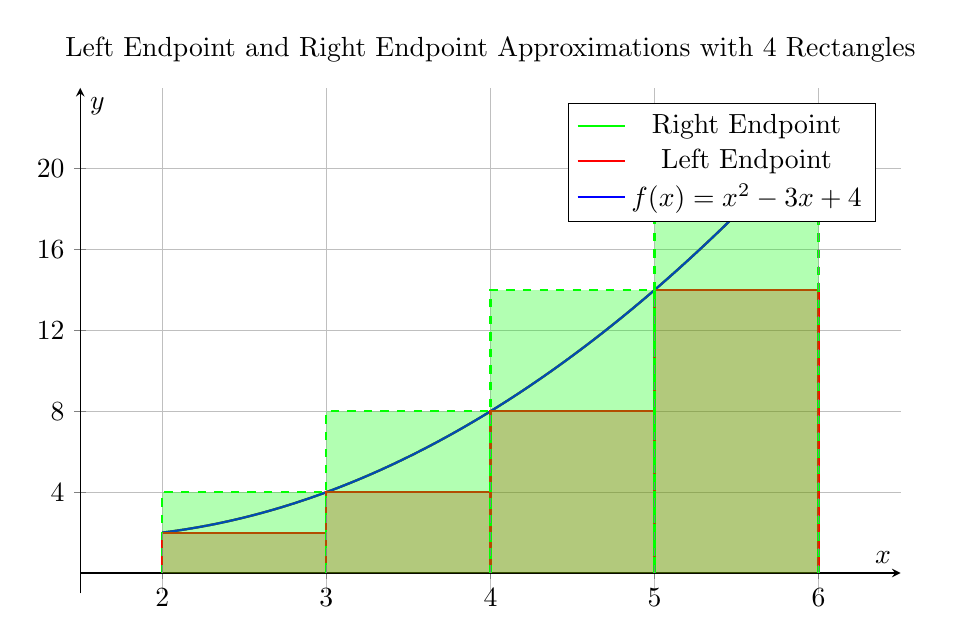
\begin{tikzpicture}
\begin{axis}[
    width=12cm,
    height=8cm,
    axis lines=middle,
    xlabel=$x$,
    ylabel=$y$,
    xmin=1.5,
    xmax=6.5,
    ymin=-1,
    ymax=24,
    xtick={2,3,4,5,6},
    ytick={0,4,8,12,16,20},
    grid=major,
    legend pos=north east,
    title={Left Endpoint and Right Endpoint Approximations with 4 Rectangles}
]

% Function plot
\addplot[domain=2:6, samples=100, thick, green] {x^2 - 3*x + 4} node[left] {$f(x) = x^2 - 3x + 4$};
\addplot[domain=2:6, samples=100, thick, red] {x^2 - 3*x + 4} node[left] {$f(x) = x^2 - 3x + 4$};
\addplot[domain=2:6, samples=100, thick, blue] {x^2 - 3*x + 4} node[left] {$f(x) = x^2 - 3x + 4$};

% Calculate partition points
\pgfmathsetmacro{\dx}{(6-2)/4}
\pgfmathsetmacro{\xa}{2}
\pgfmathsetmacro{\xb}{2+\dx}
\pgfmathsetmacro{\xc}{2+2*\dx}
\pgfmathsetmacro{\xd}{2+3*\dx}
\pgfmathsetmacro{\xe}{6}

% Calculate function values at partition points
\pgfmathsetmacro{\ya}{(\xa)^2 - 3*(\xa) + 4}
\pgfmathsetmacro{\yb}{(\xb)^2 - 3*(\xb) + 4}
\pgfmathsetmacro{\yc}{(\xc)^2 - 3*(\xc) + 4}
\pgfmathsetmacro{\yd}{(\xd)^2 - 3*(\xd) + 4}
\pgfmathsetmacro{\ye}{(\xe)^2 - 3*(\xe) + 4}

% Left endpoint rectangles
\addplot[const plot, fill=red, fill opacity=0.3, draw=red, thick]
    coordinates {
        (\xa,0) (\xa,\ya) (\xb,\ya) (\xb,0)
    };
\addplot[const plot, fill=red, fill opacity=0.3, draw=red, thick]
    coordinates {
        (\xb,0) (\xb,\yb) (\xc,\yb) (\xc,0)
    };
\addplot[const plot, fill=red, fill opacity=0.3, draw=red, thick]
    coordinates {
        (\xc,0) (\xc,\yc) (\xd,\yc) (\xd,0)
    };
\addplot[const plot, fill=red, fill opacity=0.3, draw=red, thick]
    coordinates {
        (\xd,0) (\xd,\yd) (\xe,\yd) (\xe,0)
    };

% Right endpoint rectangles
\addplot[const plot, fill=green, fill opacity=0.3, draw=green, thick, dashed]
    coordinates {
        (\xa,0) (\xa,\yb) (\xb,\yb) (\xb,0)
    };
\addplot[const plot, fill=green, fill opacity=0.3, draw=green, thick, dashed]
    coordinates {
        (\xb,0) (\xb,\yc) (\xc,\yc) (\xc,0)
    };
\addplot[const plot, fill=green, fill opacity=0.3, draw=green, thick, dashed]
    coordinates {
        (\xc,0) (\xc,\yd) (\xd,\yd) (\xd,0)
    };
\addplot[const plot, fill=green, fill opacity=0.3, draw=green, thick, dashed]
    coordinates {
        (\xd,0) (\xd,\ye) (\xe,\ye) (\xe,0)
    };

% Legend
\addlegendentry{Right Endpoint}
\addlegendentry{Left Endpoint}
\addlegendentry{$f(x) = x^2 - 3x + 4$}



% Marking the subintervals with vertical lines
\draw [gray, dashed] (axis cs:\xa,0) -- (axis cs:\xa,\ya);
\draw [gray, dashed] (axis cs:\xb,0) -- (axis cs:\xb,\yb);
\draw [gray, dashed] (axis cs:\xc,0) -- (axis cs:\xc,\yc);
\draw [gray, dashed] (axis cs:\xd,0) -- (axis cs:\xd,\yd);
\draw [gray, dashed] (axis cs:\xe,0) -- (axis cs:\xe,\ye);

\end{axis}
\end{tikzpicture}


\section*{Answer of Q4}
We want to find the Riemann sum for the function 
\[
f(x) = 4 - x^2
\]
over the interval \([-1,2]\) corresponding to the partition:
\[
x_0 = -1, \quad x_1 = 0, \quad x_2 = \frac{1}{2}, \quad x_3 = \frac{5}{4}, \quad x_4 = 2
\]
with sample points:
\[
x_1^* = -\frac{1}{4}, \quad x_2^* = \frac{1}{4}, \quad x_3^* = 1, \quad x_4^* = \frac{5}{4}.
\]

\subsection*{Step 1: Compute \(\Delta x_i\)}
The width of each subinterval is:
\[
\Delta x_1 = x_1 - x_0 = 0 - (-1) = 1
\]
\[
\Delta x_2 = x_2 - x_1 = \frac{1}{2} - 0 = \frac{1}{2}
\]
\[
\Delta x_3 = x_3 - x_2 = \frac{5}{4} - \frac{1}{2} = \frac{3}{4}
\]
\[
\Delta x_4 = x_4 - x_3 = 2 - \frac{5}{4} = \frac{3}{4}.
\]

\subsection*{Step 2: Evaluate \( f(x_i^*) \)}
Evaluate the function at each sample point:
\[
f\left(-\frac{1}{4}\right) = 4 - \left(-\frac{1}{4}\right)^2 = 4 - \frac{1}{16} = \frac{63}{16}
\]
\[
f\left(\frac{1}{4}\right) = 4 - \left(\frac{1}{4}\right)^2 = 4 - \frac{1}{16} = \frac{63}{16}
\]
\[
f(1) = 4 - 1 = 3
\]
\[
f\left(\frac{5}{4}\right) = 4 - \left(\frac{5}{4}\right)^2 = 4 - \frac{25}{16} = \frac{39}{16}.
\]

\subsection*{Step 3: Compute the Riemann Sum}
The Riemann sum is given by:
\[
S = \sum_{i=1}^{4} f(x_i^*) \Delta x_i
\]

Substituting the values:
\[
S = \left(\frac{63}{16} \times 1\right) + \left(\frac{63}{16} \times \frac{1}{2}\right) + \left(3 \times \frac{3}{4}\right) + \left(\frac{39}{16} \times \frac{3}{4}\right).
\]

Evaluating each term:
\[
\frac{63}{16} \times 1 = \frac{63}{16}
\]
\[
\frac{63}{16} \times \frac{1}{2} = \frac{63}{32}
\]
\[
3 \times \frac{3}{4} = \frac{9}{4}
\]
\[
\frac{39}{16} \times \frac{3}{4} = \frac{117}{64}.
\]

\subsection*{Step 4: Combine the Results}
Converting all fractions to a common denominator of 64:
\[
\frac{63}{16} = \frac{252}{64}, \quad \frac{63}{32} = \frac{126}{64}, \quad \frac{9}{4} = \frac{144}{64}, \quad \frac{117}{64} \text{ remains unchanged.}
\]

Thus:
\[
S \approx \frac{252}{64} + \frac{126}{64} + \frac{144}{64} + \frac{117}{64} = \frac{639}{64}.
\]

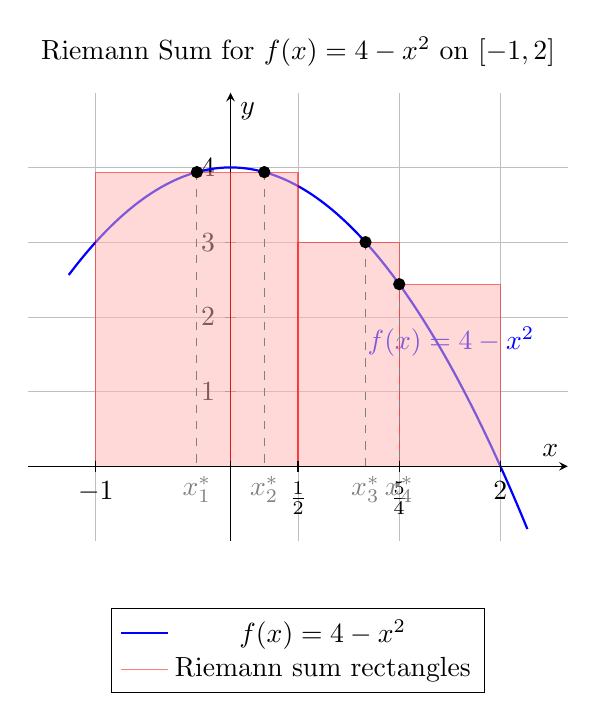
\begin{tikzpicture}
\begin{axis}[
    axis lines=middle,
    xlabel=$x$,
    ylabel=$y$,
    xmin=-1.5, xmax=2.5,
    ymin=-1, ymax=5,
    xtick={-1,0,0.5,1.25,2},
    xticklabels={$-1$,$0$,$\frac{1}{2}$,$\frac{5}{4}$,$2$},
    ytick={0,1,2,3,4},
    grid=both,
    grid style={line width=.1pt, draw=gray!10},
    major grid style={line width=.2pt,draw=gray!50},
    title={Riemann Sum for $f(x) = 4 - x^2$ on $[-1,2]$},
    legend style={at={(0.5,-0.15)}, anchor=north},
    samples=100,
    domain=-1.2:2.2,
]

% Plot the function
\addplot[blue, thick, smooth] {4 - x^2} node[pos=0.7, above] {$f(x) = 4 - x^2$};

% Define sample points
\pgfmathsetmacro{\xa}{-0.25}
\pgfmathsetmacro{\xb}{0.25}
\pgfmathsetmacro{\xc}{1}
\pgfmathsetmacro{\xd}{1.25}

% Calculate function values at sample points
\pgfmathsetmacro{\fa}{4 - (\xa)^2}
\pgfmathsetmacro{\fb}{4 - (\xb)^2}
\pgfmathsetmacro{\fc}{4 - (\xc)^2}
\pgfmathsetmacro{\fd}{4 - (\xd)^2}

% Draw rectangles for the Riemann sum
\addplot[fill=red!30, draw=red, opacity=0.5] coordinates {(-1,0) (-1,\fa) (0,\fa) (0,0)};
\addplot[fill=red!30, draw=red, opacity=0.5] coordinates {(0,0) (0,\fb) (0.5,\fb) (0.5,0)};
\addplot[fill=red!30, draw=red, opacity=0.5] coordinates {(0.5,0) (0.5,\fc) (1.25,\fc) (1.25,0)};
\addplot[fill=red!30, draw=red, opacity=0.5] coordinates {(1.25,0) (1.25,\fd) (2,\fd) (2,0)};

% Mark partition points on x-axis
\addplot[mark=|, black, mark size=2pt] coordinates {(-1,0) (0,0) (0.5,0) (1.25,0) (2,0)};

% Mark sample points and their function values
\addplot[mark=*, mark options={fill=black}, only marks] coordinates {
    (\xa,\fa) (\xb,\fb) (\xc,\fc) (\xd,\fd)
};

% Draw dashed lines from sample points to axes
\draw[dashed, gray] (axis cs:\xa,\fa) -- (axis cs:\xa,0) node[below] {$x_1^*$};
\draw[dashed, gray] (axis cs:\xb,\fb) -- (axis cs:\xb,0) node[below] {$x_2^*$};
\draw[dashed, gray] (axis cs:\xc,\fc) -- (axis cs:\xc,0) node[below] {$x_3^*$};
\draw[dashed, gray] (axis cs:\xd,\fd) -- (axis cs:\xd,0) node[below] {$x_4^*$};

% Add legend
\addlegendentry{$f(x) = 4 - x^2$}
\addplot[red!30, opacity=0.5] coordinates {(0,0) (0,0)}; 
\addlegendentry{Riemann sum rectangles}

\end{axis}
\end{tikzpicture}
\section*{Answer of Q5}
\subsection*{(a)}
The area under the curve can be expressed as a limit of Riemann sums:

\[
\lim_{n \to \infty} \sum_{k=1}^{n} f(x_k) \Delta x
\]

\textbf{Step 1: Define the partition.}  
\[
a = 0, \quad b = 2, \quad \Delta x = \frac{b-a}{n} = \frac{2-0}{n} = \frac{2}{n}
\]
\[
x_k = a + k \Delta x = 0 + k \cdot \frac{2}{n} = \frac{2k}{n}
\]

\textbf{Step 2: Write the Riemann sum.}  
\[
\lim_{n \to \infty} \sum_{k=1}^{n} f\left( \frac{2k}{n} \right) \Delta x
\]

Substitute $f(x) = x^3 + x$:
\[
= \lim_{n \to \infty} \sum_{k=1}^{n} \left[ \left(\frac{2k}{n}\right)^3 + \frac{2k}{n} \right] \cdot \frac{2}{n}
\]

\textbf{Step 3: Simplify the expression.}
\[
= \lim_{n \to \infty} \sum_{k=1}^{n} \left[ \frac{8k^3}{n^3} + \frac{2k}{n} \right] \cdot \frac{2}{n}
\]
\[
= \lim_{n \to \infty} \sum_{k=1}^{n} \left( \frac{16k^3}{n^4} + \frac{4k}{n^2} \right)
\]

\textbf{Step 4: Separate the sums.}
\[
= \lim_{n \to \infty} \left[ \frac{16}{n^4} \sum_{k=1}^{n} k^3 + \frac{4}{n^2} \sum_{k=1}^{n} k \right]
\]

\textbf{Step 5: Use known summation formulas.}
\[
\sum_{k=1}^{n} k = \frac{n(n+1)}{2}, \quad \sum_{k=1}^{n} k^3 = \left( \frac{n(n+1)}{2} \right)^2
\]

Substitute these into the expression:
\[
= \lim_{n \to \infty} \left[ \frac{16}{n^4} \left( \frac{n^2(n+1)^2}{4} \right) + \frac{4}{n^2} \cdot \frac{n(n+1)}{2} \right]
\]

\textbf{Step 6: Simplify each term.}
\[
= \lim_{n \to \infty} \left[ \frac{4(n+1)^2}{n^2} + \frac{2(n+1)}{n} \right]
\]

\textbf{Step 7: Expand and combine like terms.}
\[
= \lim_{n \to \infty} \left[ \frac{4(n^2 + 2n + 1)}{n^2} + \frac{2(n+1)}{n} \right]
\]
\[
= \lim_{n \to \infty} \left( 4 + \frac{8}{n} + \frac{4}{n^2} + 2 + \frac{2}{n} \right)
\]
\subsection*{(b)}
We will approximate this integral using a Riemann sum.

\subsubsection*{Step 1: Partitioning the Interval}
Let the interval \([0, \pi]\) be divided into \(n\) subintervals of equal length. Then:
\[
a = 0, \quad b = \pi, \quad \Delta x = \frac{\pi}{n}.
\]

\subsubsection*{Step 2: Choosing Sample Points}
We choose the right endpoints for the subintervals as the sample points:
\[
x_k = a + k\Delta x = 0 + k \cdot \frac{\pi}{n} = \frac{k\pi}{n}, \quad \text{for } k = 1, 2, \dots, n.
\]



\subsubsection*{Step 3: Expressing the Area as a Limit}
To find the exact area, we take the limit of the Riemann sum as \(n \to \infty\):
\[
\lim_{n \to \infty} \sum_{k=1}^{n} f(x_k) \Delta x = \lim_{n \to \infty} \sum_{k=1}^{n} \sqrt{\sin\left(\frac{k\pi}{n}\right)} \cdot \frac{\pi}{n}.
\]

Factoring out the constant \(\frac{\pi}{n}\), we get:
\[
= \lim_{n \to \infty} \frac{\pi}{n} \sum_{k=1}^{n} \sqrt{\sin\left(\frac{k\pi}{n}\right)}.
\]

\subsection*{(c)}
To find the area under the curve as a limit, we use the definition of a definite integral in terms of Riemann sums:
\\
\[
\lim_{n \to \infty} \sum_{k=1}^{n} f(x_k^{*}) \Delta x
\]

\subsubsection*{Step 1: Identify the Interval and Partition}
Given:
\\
\[
 a = -2, \quad b = 0
\]
The width of each subinterval ($\Delta x$) is:
\\
\[
\Delta x = \frac{b - a}{n} = \frac{0 - (-2)}{n} = \frac{2}{n}
\]

\subsubsection*{Step 2: Determine the Sample Points}

For a left-endpoint Riemann sum, we choose the sample points:
\\
\[
x_{n-k} = b - k\Delta x = 0 - k \cdot \frac{2}{n} = -\frac{2k}{n}
\]

\subsubsection*{Step 3: Write the Riemann Sum}
Realize that:\\
\[
\sum_{i=1}^na_{i-1}=\sum_{i=1}^na_{n-i}
\]
Then Riemann sum becomes:
\\
\[
\lim_{n \to \infty} \sum_{k=1}^{n} f(x_{n-k}) \Delta x
\]

Substituting $f(x) = x^2 - 3x$:
\\
\[
\lim_{n \to \infty} \sum_{k=1}^{n} \left[ \left(-\frac{2k}{n}\right)^2 - 3\left(-\frac{2k}{n}\right) \right] \cdot \frac{2}{n}
\]

\subsubsection*{Step 4: Simplify the Expression}

First, expand and simplify inside the sum:
\\
\begin{align*}
\left(-\frac{2k}{n}\right)^2 &= \frac{4k^2}{n^2} \\
-3\left(-\frac{2k}{n}\right) &= \frac{6k}{n}
\end{align*}

Thus, the sum becomes:
\\
\[
\lim_{n \to \infty} \sum_{k=1}^{n} \left( \frac{4k^2}{n^2} + \frac{6k}{n} \right) \cdot \frac{2}{n}
\]

Factor and combine like terms:
\\
\[
= \lim_{n \to \infty} \frac{2}{n} \sum_{k=1}^{n} \left( \frac{4k^2}{n^2} + \frac{6k}{n} \right)
\]

\[
= \lim_{n \to \infty} \sum_{k=1}^{n} \left( \frac{8k^2}{n^3} + \frac{12k}{n^2} \right)
\]

\subsubsection*{Step 5: Use Known Summation Formulas}

Recall the standard summation formulas:
\\
\[
\sum_{k=1}^{n} k = \frac{n(n+1)}{2}
\]
\[
\sum_{k=1}^{n} k^2 = \frac{n(n+1)(2n+1)}{6}
\]

Substitute these results into the expression:
\\
\begin{align*}
\lim_{n \to \infty} \left[ \frac{8}{n^3} \cdot \frac{n(n+1)(2n+1)}{6} + \frac{12}{n^2} \cdot \frac{n(n+1)}{2} \right]
\end{align*}

\subsubsection*{Step 6: Final Limit Expression}

The final limit expression for the area under the curve is:
\\
\[
\boxed{\lim_{n \to \infty} \left( \frac{8(n+1)(2n+1)}{6n^2} + \frac{6(n+1)}{n} \right)}
\]
\subsection*{(d)}
\subsubsection*{Step 1: Define the Riemann Sum}
The area under the curve can evaluated by the limit of the Riemann sum:
\[
A = \lim_{n \to \infty} \sum_{k=1}^{n} f(x_k) \Delta x
\]
where:
\begin{itemize}
    \item $a = 0$ and $b = 1$ represent the interval $[0,1]$.
    \item $\Delta x = \frac{b - a}{n} = \frac{1}{n}$ is the width of each subinterval.
    \item $x_k = a + k \Delta x = \frac{k}{n}$ represents the right endpoint of each subinterval.
\end{itemize}

\subsubsection*{Step 2: Substitute the Function $f(x)$}
Given the function:
\[
f(x) = \sin\left(\frac{\pi}{2} x\right),
\]
the Riemann sum becomes:
\[
A = \lim_{n \to \infty}\sum_{k=1}^{n} \sin\left(\frac{\pi}{2} \cdot \frac{k}{n}\right) \cdot \frac{1}{n}.
\]
\section*{Answer of Q6}


\[
A = \lim_{n \to \infty}\Delta x \sum_{k=1}^{n} f(x_k)  =\lim_{n \to \infty} \frac{2}{n} \sum_{k=1}^{n} \left( 5 + \frac{2k}{n} \right)^{10}
\]

\begin{itemize}
    \item Step size: \(\Delta x = \frac{2}{n}\)
    \item Sample points: \(x_k = a + k\Delta x = 5 + \frac{2k}{n}\)
    \item Interval: \([5, 7]\)
    \item Function: \(f(x) = x^{10}\)
\end{itemize}
\section*{Answer of Q7}

\noindent
\textbf{Step 1: Recognize the Increasing Nature of the Function}

The given function is:
\[
f(x) = x^4 + 1.
\]

The derivative is:
\[
f'(x) = 4x^3.
\]

Since \(f'(x) \geq 0\) for \(x \in [0,1]\), the function \(f(x)\) is increasing on the interval \([0,1]\).

\vspace{0.5cm}
\noindent
\textbf{Step 2: Applying the Lower and Upper Sum Approximations}

For an increasing function on \([0,1]\), the following inequality holds for any partition:
\[
L_n \leq A \leq R_n,
\]
where \(L_n\) is the left Riemann sum and \(R_n\) is the right Riemann sum.

We choose \(n = 3\) subintervals for the partition.

\[
\Delta x = \frac{1-0}{3} = \frac{1}{3}.
\]

\vspace{0.5cm}
\noindent
\textbf{Step 3: Compute the Left Riemann Sum \(L_3\)}

The left Riemann sum is:
\[
L_3 = \sum_{k=0}^{2} f\left(\frac{k}{3}\right) \Delta x.
\]

Substituting the values:
\[
L_3 = \frac{1}{3} \left[ f(0) + f\left(\frac{1}{3}\right) + f\left(\frac{2}{3}\right) \right].
\]

Evaluating each term:
\[
f(0) = 0^4 + 1 = 1,
\]
\[
f\left(\frac{1}{3}\right) = \left(\frac{1}{3}\right)^4 + 1 = \frac{1}{81} + 1 = \frac{82}{81},
\]
\[
f\left(\frac{2}{3}\right) = \left(\frac{2}{3}\right)^4 + 1 = \frac{16}{81} + 1 = \frac{97}{81}.
\]

Thus:
\[
L_3 = \frac{1}{3} \left[1 + \frac{82}{81} + \frac{97}{81}\right] = \frac{1}{3} \times \frac{260}{81} = \frac{260}{243} \approx 1.07.
\]

\vspace{0.5cm}
\noindent
\textbf{Step 4: Compute the Right Riemann Sum \(R_3\)}

The right Riemann sum is:
\[
R_3 = \sum_{k=1}^{3} f\left(\frac{k}{3}\right) \Delta x.
\]

Substituting the values:
\[
R_3 = \frac{1}{3} \left[ f\left(\frac{1}{3}\right) + f\left(\frac{2}{3}\right) + f(1) \right].
\]

Evaluating the last term:
\[
f(1) = 1^4 + 1 = 2.
\]

So:
\[
R_3 = \frac{1}{3} \left[\frac{82}{81} + \frac{97}{81} + 2\right] = \frac{1}{3} \times \frac{341}{81} = \frac{341}{243} \approx 1.40.
\]

\vspace{0.5cm}
\noindent
\textbf{Step 5: Conclude the Bounds for the Area \(A\)}

Since \(f(x)\) is increasing:
\[
L_3 \leq A \leq R_3.
\]

Substituting the calculated values:
\[
1.07 \leq A \leq 1.40.
\]

Thus, we have:
\[
1 < A < 1.5.
\]

\vspace{0.5cm}
\noindent
\textbf{Final Answer:} \(\boxed{\text{True}}\)


\section*{Answer of Q8}

Check the validity of:
\[
\sum_{i=1}^{n} \left( i + \sin\left(\frac{i\pi}{2}\right) \right) 
= \frac{n(n+1)}{2} + \sin\left( \frac{(n+1)\pi}{4} \right)
\]

\subsection*{Counterexample: $n=2$}

\textbf{LHS:}
\[
1 + \sin\left(\frac{\pi}{2}\right) + 2 + \sin(\pi) = 1 + 1 + 2 + 0 = 4
\]
\noindent
\textbf{RHS:}
\[
\frac{2 \times 3}{2} + \sin\left(\frac{3\pi}{4}\right) = 3 + \frac{\sqrt{2}}{2} \approx 3.707
\]

\subsection*{Conclusion}



Since:
\[
\text{LHS} = 4 \neq \text{RHS} \approx 3.707
\]

The equation is \textbf{false}.
\section*{Answer of Q9}
\subsection*{Problem Statement}
Let $A$ be the area under the graph of an increasing continuous function $f$ from $a$ to $b$. Let $L_n$ and $R_n$ be the approximations to $A$ with $n$ subintervals using left and right endpoints, respectively.

\begin{enumerate}
    \item[(a)] How are $A$, $L_n$, and $R_n$ related?
    \item[(b)] Show that $R_n - L_n = \dfrac{b - a}{n}\bigl[f(b) - f(a)\bigr]$.
\end{enumerate}

\subsection*{(a) Relationship between $A$, $L_n$, and $R_n$}
Since $f$ is increasing and continuous on the interval $[a,b]$:

\begin{itemize}
    \item $L_n$ (Left Riemann Sum) gives a \textbf{lower estimation} for $A$, because it uses the function values at the left endpoints, which are always less than or equal to the function values at the right endpoints in the case of an increasing function.
    \item $R_n$ (Right Riemann Sum) gives an \textbf{upper estimation} for $A$, since it uses the function values at the right endpoints, which are greater than or equal to the function values at the left endpoints.
\end{itemize}

Thus, the area $A$ will be bounded by $L_n$ and $R_n$ as follows:
\[
L_n \leq A \leq R_n, \quad \text{for all natural numbers } n.
\]

\subsection*{(b) Proof that $R_n - L_n = \dfrac{b - a}{n}[f(b) - f(a)]$}

\subsubsection*{Step 1: Recall Definitions}
Let $\Delta x = \dfrac{b - a}{n}$ and partition the interval $[a, b]$ into $n$ equal subintervals. Define the points:
\[
    x_k = a + k\Delta x, \quad k = 0, 1, 2, \ldots, n.
\]

The right Riemann sum ($R_n$) and left Riemann sum ($L_n$) are defined as:
\begin{align*}
    R_n &= \sum_{k=1}^{n} f(x_k) \Delta x, \\
    L_n &= \sum_{k=0}^{n-1} f(x_k) \Delta x.
\end{align*}

\subsubsection*{Step 2: Compute $R_n - L_n$}
\begin{align*}
    R_n - L_n &=  \sum_{k=1}^{n} f(x_k)\Delta x - \sum_{k=0}^{n-1} f(x_k)\Delta x \\
    &=\Delta x \left[ \sum_{k=1}^{n} f(x_k) - \sum_{k=0}^{n-1} f(x_k) \right]\\
    &=\Delta x \left[ \sum_{k=1}^{n-1} f(x_k) + f(x_n) - f(x_0) - \sum_{k=1}^{n-1} f(x_k) \right].
\end{align*}

Notice that most terms cancel out in the subtraction, leaving:
\begin{align*}
    R_n - L_n &= \Delta x \bigl[f(x_n) - f(x_0)\bigr].
\end{align*}

Since $x_n = b$ and $x_0 = a$, this becomes:
\begin{align*}
    R_n - L_n &= \Delta x \bigl[f(b) - f(a)\bigr].
\end{align*}

Substituting $\Delta x = \dfrac{b - a}{n}$:
\begin{align*}
    R_n - L_n &= \frac{b - a}{n}\bigl[f(b) - f(a)\bigr].
\end{align*}

\subsubsection*{Step 3: Final Result}
We have shown that:
\[
    R_n - L_n = \frac{b - a}{n}\bigl[f(b) - f(a)\bigr].
\]

\subsubsection*{Step 4: Proof that $x_n=b$}
To confirm the expression for $x_n$:
\begin{align*}
    x_n &= a + n\Delta x \\
        &= a + n\frac{b - a}{n} \\
        &= a + b - a \\
        &= b.
\end{align*}

This verifies that the endpoint calculations are consistent.



\section*{About The Repository}

This document is part of the \href{https://github.com/3ndlyb/Math132Answers}{\texttt{github.com/3ndlyb/Math132Answers}} repository, which contains solutions to Math132 problem sheets. Each sheet is organized in its own folder, including:

\begin{itemize}
    \item The original problem sheet in PDF format (\texttt{Math - 132 - sheetX.pdf}).
    \item A \LaTeX{} source file (\texttt{main.tex}) containing the answers.
    \item The compiled PDF of the answers (\texttt{SheetXAns.pdf}).
\end{itemize}

To view the answers, simply open the corresponding \texttt{SheetXAns.pdf} file. If you wish to edit the answers, you can modify the \texttt{main.tex} file and recompile it using:

\begin{tcolorbox}[terminal]
\begin{verbatim}
$ pdflatex main.tex
\end{verbatim}
\end{tcolorbox}


Make sure you have a suitable \LaTeX{} distribution installed, such as TeX Live or MiKTeX.

\subsection*{Contributions and Feedback}

Contributions to improve the repository are welcome. If you spot any errors or have suggestions, feel free to:
\begin{enumerate}
    \item Open an issue on the GitHub repository.
    \item Fork the repository, make your changes, and submit a pull request.
\end{enumerate}

The repository is licensed under the MIT License, so you are free to use, modify, and share the materials.  

\subsection*{Contact}

For further questions or feedback, feel free to reach out via Discord at \boxed{\texttt{3ndlybalabyd}} \! .
\definecolor{spotifygreen}{RGB}{30,215,96} % Official Spotify Green

\section*{Acknowledgments}

\begin{tcolorbox}[
    colback=black,         % Background color
    colframe=spotifygreen, % Border color (Spotify green)
    width=\textwidth,      % Full width
    boxrule=1mm,           % Border thickness
    sharp corners=south,   % Rounded top corners only
    arc=5mm,               % Curve radius for corners
    fontupper=\color{white}\sffamily, % White sans-serif text
    title=\textbf{\huge \textcolor{white}{\faSpotify} Spotify Playlist},
    coltitle=white,        % Title text color
    attach boxed title to top left={yshift=-2mm, xshift=5mm},
    boxed title style={colback=black, sharp corners}
]
    \begin{center}
        % ------ PLAYLIST COVER IMAGE ------
        
\includegraphics[width=4cm,clip,trim=0 0 0 0]{playlist_cover.jpg}

        \vspace{0.5cm}

        % ------ DESCRIPTION ------
        This document wouldn't have been possible without my beloved Spotify playlist.\\ Click the link below or scan the QR code to listen to it:

        \vspace{0.5cm}

        % ------ CLICKABLE LINK ------
        \href{https://open.spotify.com/playlist/5iKzfelUIiTW2IHZWqRzKC}{%
            \textcolor{spotifygreen}{\Large \textbf{Listen on Spotify}}%
        }

        \vspace{0.5cm}

        % ------ QR CODE ------
        \qrcode[height=3cm]{https://open.spotify.com/playlist/5iKzfelUIiTW2IHZWqRzKC}
    \end{center}
\end{tcolorbox}

\end{document}
